\documentclass[10pt]{standalone}
\usepackage{pgfplots}
\pgfplotsset{compat=1.15}
\usepackage{mathrsfs}
\usepackage{amssymb}
\usepackage{amsmath}
\usepackage{anyfontsize}
\usetikzlibrary{arrows}
\pagestyle{empty}

\begin{document}



\tikzset{every picture/.style={line width=0.75pt}} %set default line width to 0.75pt        

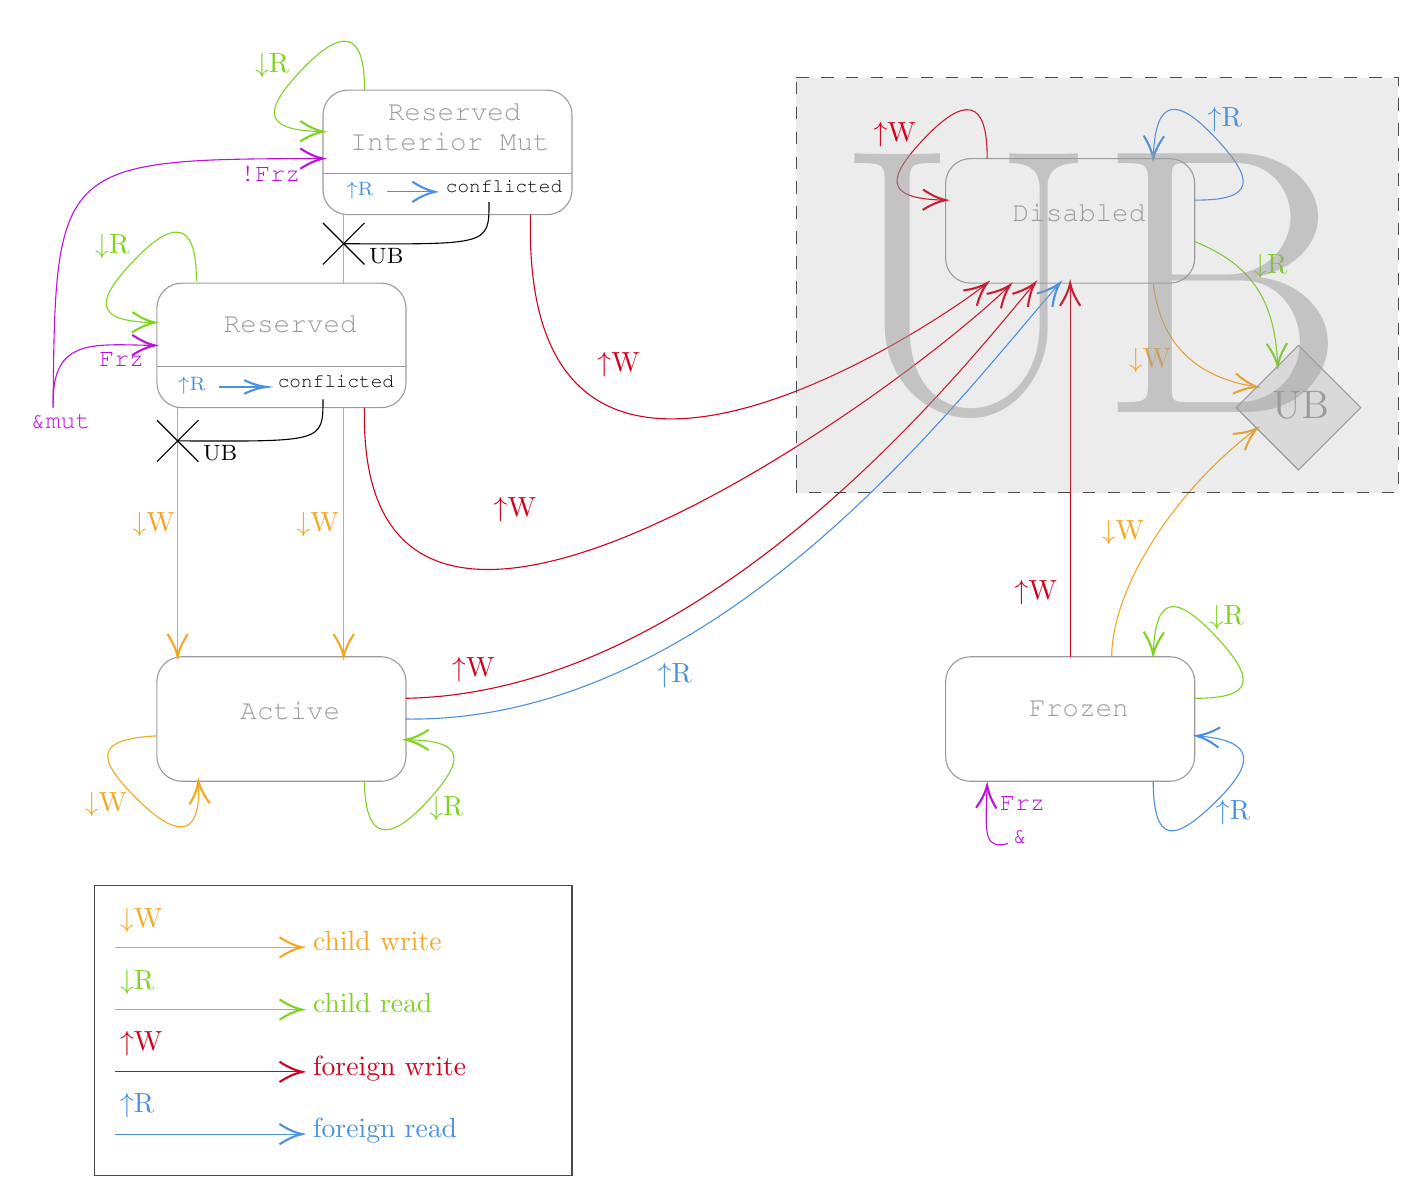
\begin{tikzpicture}[x=0.75pt,y=0.75pt,yscale=-1,xscale=1]
%uncomment if require: \path (0,618); %set diagram left start at 0, and has height of 618

%Rounded Rect [id:dp6273975077546735] 
\draw  [color={rgb, 255:red, 155; green, 155; blue, 155 }  ,draw opacity=1 ] (80,132) .. controls (80,125.37) and (85.37,120) .. (92,120) -- (188,120) .. controls (194.63,120) and (200,125.37) .. (200,132) -- (200,168) .. controls (200,174.63) and (194.63,180) .. (188,180) -- (92,180) .. controls (85.37,180) and (80,174.63) .. (80,168) -- cycle ;
%Straight Lines [id:da054054294625888843] 
\draw [color={rgb, 255:red, 155; green, 155; blue, 155 }  ,draw opacity=1 ]   (80,160) -- (200,160) ;
%Rounded Rect [id:dp32196207672856103] 
\draw  [color={rgb, 255:red, 155; green, 155; blue, 155 }  ,draw opacity=1 ] (80,312) .. controls (80,305.37) and (85.37,300) .. (92,300) -- (188,300) .. controls (194.63,300) and (200,305.37) .. (200,312) -- (200,348) .. controls (200,354.63) and (194.63,360) .. (188,360) -- (92,360) .. controls (85.37,360) and (80,354.63) .. (80,348) -- cycle ;
%Rounded Rect [id:dp2083188670445868] 
\draw  [color={rgb, 255:red, 155; green, 155; blue, 155 }  ,draw opacity=1 ] (460,72) .. controls (460,65.37) and (465.37,60) .. (472,60) -- (568,60) .. controls (574.63,60) and (580,65.37) .. (580,72) -- (580,108) .. controls (580,114.63) and (574.63,120) .. (568,120) -- (472,120) .. controls (465.37,120) and (460,114.63) .. (460,108) -- cycle ;
%Rounded Rect [id:dp03888310762724445] 
\draw  [color={rgb, 255:red, 155; green, 155; blue, 155 }  ,draw opacity=1 ] (460,312) .. controls (460,305.37) and (465.37,300) .. (472,300) -- (568,300) .. controls (574.63,300) and (580,305.37) .. (580,312) -- (580,348) .. controls (580,354.63) and (574.63,360) .. (568,360) -- (472,360) .. controls (465.37,360) and (460,354.63) .. (460,348) -- cycle ;
%Straight Lines [id:da8884245902951894] 
\draw [color={rgb, 255:red, 208; green, 2; blue, 27 }  ,draw opacity=1 ]   (520,300) -- (520,122) ;
\draw [shift={(520,120)}, rotate = 90] [color={rgb, 255:red, 208; green, 2; blue, 27 }  ,draw opacity=1 ][line width=0.75]    (10.93,-4.9) .. controls (6.95,-2.3) and (3.31,-0.67) .. (0,0) .. controls (3.31,0.67) and (6.95,2.3) .. (10.93,4.9)   ;
%Curve Lines [id:da2912349258531959] 
\draw [color={rgb, 255:red, 208; green, 2; blue, 27 }  ,draw opacity=1 ]   (200,320) .. controls (346.76,317.38) and (470.36,158.67) .. (502.07,121.1) ;
\draw [shift={(503,120)}, rotate = 130.38] [color={rgb, 255:red, 208; green, 2; blue, 27 }  ,draw opacity=1 ][line width=0.75]    (10.93,-4.9) .. controls (6.95,-2.3) and (3.31,-0.67) .. (0,0) .. controls (3.31,0.67) and (6.95,2.3) .. (10.93,4.9)   ;
%Curve Lines [id:da3819617948887055] 
\draw [color={rgb, 255:red, 126; green, 211; blue, 33 }  ,draw opacity=1 ]   (580,100) .. controls (608.33,111.28) and (618.5,129.43) .. (619.92,158.22) ;
\draw [shift={(620,160)}, rotate = 267.91] [color={rgb, 255:red, 126; green, 211; blue, 33 }  ,draw opacity=1 ][line width=0.75]    (10.93,-4.9) .. controls (6.95,-2.3) and (3.31,-0.67) .. (0,0) .. controls (3.31,0.67) and (6.95,2.3) .. (10.93,4.9)   ;
%Curve Lines [id:da8535455424104158] 
\draw [color={rgb, 255:red, 245; green, 166; blue, 35 }  ,draw opacity=1 ]   (560,120) .. controls (562.87,143.82) and (575.2,164.22) .. (608.47,169.76) ;
\draw [shift={(610,170)}, rotate = 188.52] [color={rgb, 255:red, 245; green, 166; blue, 35 }  ,draw opacity=1 ][line width=0.75]    (10.93,-4.9) .. controls (6.95,-2.3) and (3.31,-0.67) .. (0,0) .. controls (3.31,0.67) and (6.95,2.3) .. (10.93,4.9)   ;
%Straight Lines [id:da24180993042800214] 
\draw [color={rgb, 255:red, 245; green, 166; blue, 35 }  ,draw opacity=1 ]   (90,180) -- (90,298) ;
\draw [shift={(90,300)}, rotate = 270] [color={rgb, 255:red, 245; green, 166; blue, 35 }  ,draw opacity=1 ][line width=0.75]    (10.93,-4.9) .. controls (6.95,-2.3) and (3.31,-0.67) .. (0,0) .. controls (3.31,0.67) and (6.95,2.3) .. (10.93,4.9)   ;
%Curve Lines [id:da40732512812928434] 
\draw [color={rgb, 255:red, 245; green, 166; blue, 35 }  ,draw opacity=1 ]   (540,300) .. controls (540.24,267.18) and (569.41,220.94) .. (608.8,190.91) ;
\draw [shift={(610,190)}, rotate = 143.13] [color={rgb, 255:red, 245; green, 166; blue, 35 }  ,draw opacity=1 ][line width=0.75]    (10.93,-4.9) .. controls (6.95,-2.3) and (3.31,-0.67) .. (0,0) .. controls (3.31,0.67) and (6.95,2.3) .. (10.93,4.9)   ;
%Curve Lines [id:da3211866387795047] 
\draw [color={rgb, 255:red, 74; green, 144; blue, 226 }  ,draw opacity=1 ]   (560,360) .. controls (560.24,390.84) and (570.42,389.16) .. (590,370) .. controls (609.19,351.23) and (609.25,340.61) .. (582.66,338.27) ;
\draw [shift={(581,338.13)}, rotate = 4.14] [color={rgb, 255:red, 74; green, 144; blue, 226 }  ,draw opacity=1 ][line width=0.75]    (10.93,-4.9) .. controls (6.95,-2.3) and (3.31,-0.67) .. (0,0) .. controls (3.31,0.67) and (6.95,2.3) .. (10.93,4.9)   ;
%Curve Lines [id:da7740088126292866] 
\draw [color={rgb, 255:red, 126; green, 211; blue, 33 }  ,draw opacity=1 ]   (99,119) .. controls (99.24,89.84) and (87.91,89.18) .. (69,109) .. controls (50.46,128.43) and (49.28,138.12) .. (77.25,138.96) ;
\draw [shift={(79,139)}, rotate = 180.94] [color={rgb, 255:red, 126; green, 211; blue, 33 }  ,draw opacity=1 ][line width=0.75]    (10.93,-4.9) .. controls (6.95,-2.3) and (3.31,-0.67) .. (0,0) .. controls (3.31,0.67) and (6.95,2.3) .. (10.93,4.9)   ;
%Curve Lines [id:da45423662928532793] 
\draw [color={rgb, 255:red, 208; green, 2; blue, 27 }  ,draw opacity=1 ]   (480,60) .. controls (480.24,30.84) and (468.91,30.18) .. (450,50) .. controls (431.47,69.43) and (430.29,79.12) .. (458.25,79.96) ;
\draw [shift={(460,80)}, rotate = 180.94] [color={rgb, 255:red, 208; green, 2; blue, 27 }  ,draw opacity=1 ][line width=0.75]    (10.93,-4.9) .. controls (6.95,-2.3) and (3.31,-0.67) .. (0,0) .. controls (3.31,0.67) and (6.95,2.3) .. (10.93,4.9)   ;
%Curve Lines [id:da24160609309272352] 
\draw [color={rgb, 255:red, 74; green, 144; blue, 226 }  ,draw opacity=1 ]   (580,80) .. controls (609.58,80.18) and (608.91,70.18) .. (590,50) .. controls (571.47,30.23) and (561.32,30.81) .. (560.07,58.28) ;
\draw [shift={(560,60)}, rotate = 271.79] [color={rgb, 255:red, 74; green, 144; blue, 226 }  ,draw opacity=1 ][line width=0.75]    (10.93,-4.9) .. controls (6.95,-2.3) and (3.31,-0.67) .. (0,0) .. controls (3.31,0.67) and (6.95,2.3) .. (10.93,4.9)   ;
%Curve Lines [id:da7318947934920718] 
\draw [color={rgb, 255:red, 126; green, 211; blue, 33 }  ,draw opacity=1 ]   (580,320) .. controls (609.58,320.18) and (608.91,310.18) .. (590,290) .. controls (571.47,270.23) and (561.32,269.85) .. (560.07,297.29) ;
\draw [shift={(560,299)}, rotate = 271.79] [color={rgb, 255:red, 126; green, 211; blue, 33 }  ,draw opacity=1 ][line width=0.75]    (10.93,-4.9) .. controls (6.95,-2.3) and (3.31,-0.67) .. (0,0) .. controls (3.31,0.67) and (6.95,2.3) .. (10.93,4.9)   ;
%Curve Lines [id:da17055487107573564] 
\draw [color={rgb, 255:red, 245; green, 166; blue, 35 }  ,draw opacity=1 ]   (80,338.13) .. controls (49.58,339.64) and (50.91,348.98) .. (70,368.13) .. controls (88.71,386.91) and (101.08,388.26) .. (100.08,361.66) ;
\draw [shift={(100,360)}, rotate = 86.81] [color={rgb, 255:red, 245; green, 166; blue, 35 }  ,draw opacity=1 ][line width=0.75]    (10.93,-4.9) .. controls (6.95,-2.3) and (3.31,-0.67) .. (0,0) .. controls (3.31,0.67) and (6.95,2.3) .. (10.93,4.9)   ;
%Curve Lines [id:da8919790382326966] 
\draw [color={rgb, 255:red, 126; green, 211; blue, 33 }  ,draw opacity=1 ]   (180,360) .. controls (180.24,387.64) and (191.09,390.49) .. (210,370) .. controls (228.53,349.92) and (228.9,340.56) .. (201.7,340.02) ;
\draw [shift={(200,340)}, rotate = 0.35] [color={rgb, 255:red, 126; green, 211; blue, 33 }  ,draw opacity=1 ][line width=0.75]    (10.93,-4.9) .. controls (6.95,-2.3) and (3.31,-0.67) .. (0,0) .. controls (3.31,0.67) and (6.95,2.3) .. (10.93,4.9)   ;
%Straight Lines [id:da6717165267996893] 
\draw [color={rgb, 255:red, 126; green, 211; blue, 33 }  ,draw opacity=1 ]   (60,470) -- (148,470) ;
\draw [shift={(150,470)}, rotate = 180] [color={rgb, 255:red, 126; green, 211; blue, 33 }  ,draw opacity=1 ][line width=0.75]    (10.93,-4.9) .. controls (6.95,-2.3) and (3.31,-0.67) .. (0,0) .. controls (3.31,0.67) and (6.95,2.3) .. (10.93,4.9)   ;
%Straight Lines [id:da28312164212487456] 
\draw [color={rgb, 255:red, 245; green, 166; blue, 35 }  ,draw opacity=1 ]   (60,440) -- (148,440) ;
\draw [shift={(150,440)}, rotate = 180] [color={rgb, 255:red, 245; green, 166; blue, 35 }  ,draw opacity=1 ][line width=0.75]    (10.93,-4.9) .. controls (6.95,-2.3) and (3.31,-0.67) .. (0,0) .. controls (3.31,0.67) and (6.95,2.3) .. (10.93,4.9)   ;
%Straight Lines [id:da9644755933374497] 
\draw [color={rgb, 255:red, 208; green, 2; blue, 27 }  ,draw opacity=1 ]   (60,500) -- (148,500) ;
\draw [shift={(150,500)}, rotate = 180] [color={rgb, 255:red, 208; green, 2; blue, 27 }  ,draw opacity=1 ][line width=0.75]    (10.93,-4.9) .. controls (6.95,-2.3) and (3.31,-0.67) .. (0,0) .. controls (3.31,0.67) and (6.95,2.3) .. (10.93,4.9)   ;
%Straight Lines [id:da3937025481534393] 
\draw [color={rgb, 255:red, 74; green, 144; blue, 226 }  ,draw opacity=1 ]   (60,530) -- (148,530) ;
\draw [shift={(150,530)}, rotate = 180] [color={rgb, 255:red, 74; green, 144; blue, 226 }  ,draw opacity=1 ][line width=0.75]    (10.93,-4.9) .. controls (6.95,-2.3) and (3.31,-0.67) .. (0,0) .. controls (3.31,0.67) and (6.95,2.3) .. (10.93,4.9)   ;
%Shape: Rectangle [id:dp005076056202185875] 
\draw  [color={rgb, 255:red, 74; green, 74; blue, 74 }  ,draw opacity=1 ] (50,410) -- (280,410) -- (280,550) -- (50,550) -- cycle ;
%Curve Lines [id:da26786396298393433] 
\draw [color={rgb, 255:red, 189; green, 16; blue, 224 }  ,draw opacity=1 ]   (30,180) .. controls (28.93,146.7) and (47.97,149.43) .. (77.2,149.97) ;
\draw [shift={(79,150)}, rotate = 180.84] [color={rgb, 255:red, 189; green, 16; blue, 224 }  ,draw opacity=1 ][line width=0.75]    (10.93,-4.9) .. controls (6.95,-2.3) and (3.31,-0.67) .. (0,0) .. controls (3.31,0.67) and (6.95,2.3) .. (10.93,4.9)   ;
%Curve Lines [id:da23539814702482686] 
\draw [color={rgb, 255:red, 189; green, 16; blue, 224 }  ,draw opacity=1 ]   (490,390) .. controls (478.7,392.82) and (479.05,385.92) .. (479.93,363.74) ;
\draw [shift={(480,362)}, rotate = 92.24] [color={rgb, 255:red, 189; green, 16; blue, 224 }  ,draw opacity=1 ][line width=0.75]    (10.93,-4.9) .. controls (6.95,-2.3) and (3.31,-0.67) .. (0,0) .. controls (3.31,0.67) and (6.95,2.3) .. (10.93,4.9)   ;
%Rounded Rect [id:dp9087020644003058] 
\draw  [color={rgb, 255:red, 155; green, 155; blue, 155 }  ,draw opacity=1 ] (160,39.01) .. controls (160,32.38) and (165.37,27.01) .. (172,27.01) -- (268,27.01) .. controls (274.63,27.01) and (280,32.38) .. (280,39.01) -- (280,75.01) .. controls (280,81.63) and (274.63,87.01) .. (268,87.01) -- (172,87.01) .. controls (165.37,87.01) and (160,81.63) .. (160,75.01) -- cycle ;
%Straight Lines [id:da5844076607337373] 
\draw [color={rgb, 255:red, 155; green, 155; blue, 155 }  ,draw opacity=1 ]   (160,67.01) -- (280,67.01) ;
%Curve Lines [id:da7740127989298016] 
\draw [color={rgb, 255:red, 126; green, 211; blue, 33 }  ,draw opacity=1 ]   (180,27) .. controls (180.24,-2.16) and (168.91,-2.82) .. (150,17) .. controls (131.47,36.43) and (130.29,46.12) .. (158.25,46.96) ;
\draw [shift={(160,47)}, rotate = 180.94] [color={rgb, 255:red, 126; green, 211; blue, 33 }  ,draw opacity=1 ][line width=0.75]    (10.93,-4.9) .. controls (6.95,-2.3) and (3.31,-0.67) .. (0,0) .. controls (3.31,0.67) and (6.95,2.3) .. (10.93,4.9)   ;
%Curve Lines [id:da6270617466042688] 
\draw [color={rgb, 255:red, 189; green, 16; blue, 224 }  ,draw opacity=1 ]   (30,180) .. controls (30.91,62.61) and (32.23,60.05) .. (158.09,60) ;
\draw [shift={(160,60)}, rotate = 179.99] [color={rgb, 255:red, 189; green, 16; blue, 224 }  ,draw opacity=1 ][line width=0.75]    (10.93,-4.9) .. controls (6.95,-2.3) and (3.31,-0.67) .. (0,0) .. controls (3.31,0.67) and (6.95,2.3) .. (10.93,4.9)   ;
%Straight Lines [id:da4527840411816748] 
\draw [color={rgb, 255:red, 245; green, 166; blue, 35 }  ,draw opacity=1 ]   (170,180) -- (170,298) ;
\draw [shift={(170,300)}, rotate = 270] [color={rgb, 255:red, 245; green, 166; blue, 35 }  ,draw opacity=1 ][line width=0.75]    (10.93,-4.9) .. controls (6.95,-2.3) and (3.31,-0.67) .. (0,0) .. controls (3.31,0.67) and (6.95,2.3) .. (10.93,4.9)   ;
%Straight Lines [id:da8194793863643893] 
\draw [color={rgb, 255:red, 245; green, 166; blue, 35 }  ,draw opacity=1 ]   (170,86) -- (170,120) ;
%Straight Lines [id:da7853166712867432] 
\draw [color={rgb, 255:red, 74; green, 144; blue, 226 }  ,draw opacity=1 ]   (191,76.01) -- (212,76.01) ;
\draw [shift={(214,76.01)}, rotate = 180] [color={rgb, 255:red, 74; green, 144; blue, 226 }  ,draw opacity=1 ][line width=0.75]    (10.93,-4.9) .. controls (6.95,-2.3) and (3.31,-0.67) .. (0,0) .. controls (3.31,0.67) and (6.95,2.3) .. (10.93,4.9)   ;
%Curve Lines [id:da4441638369812718] 
\draw [color={rgb, 255:red, 208; green, 2; blue, 27 }  ,draw opacity=1 ]   (180,180) .. controls (175.87,362.53) and (436.23,174.35) .. (490.2,121.78) ;
\draw [shift={(491,121)}, rotate = 135.39] [color={rgb, 255:red, 208; green, 2; blue, 27 }  ,draw opacity=1 ][line width=0.75]    (10.93,-4.9) .. controls (6.95,-2.3) and (3.31,-0.67) .. (0,0) .. controls (3.31,0.67) and (6.95,2.3) .. (10.93,4.9)   ;
%Curve Lines [id:da008401668427480802] 
\draw [color={rgb, 255:red, 208; green, 2; blue, 27 }  ,draw opacity=1 ]   (260,87.01) .. controls (254.98,274.64) and (455.44,139.59) .. (478.58,121.18) ;
\draw [shift={(480,120)}, rotate = 138.66] [color={rgb, 255:red, 208; green, 2; blue, 27 }  ,draw opacity=1 ][line width=0.75]    (10.93,-4.9) .. controls (6.95,-2.3) and (3.31,-0.67) .. (0,0) .. controls (3.31,0.67) and (6.95,2.3) .. (10.93,4.9)   ;
%Shape: Rectangle [id:dp9138120727251573] 
\draw  [color={rgb, 255:red, 74; green, 74; blue, 74 }  ,draw opacity=1 ][fill={rgb, 255:red, 155; green, 155; blue, 155 }  ,fill opacity=0.19 ][dash pattern={on 4.5pt off 4.5pt}] (388,21) -- (678,21) -- (678,221) -- (388,221) -- cycle ;
%Shape: Diamond [id:dp8977704959731727] 
\draw  [color={rgb, 255:red, 155; green, 155; blue, 155 }  ,draw opacity=1 ][fill={rgb, 255:red, 155; green, 155; blue, 155 }  ,fill opacity=0.23 ] (630,150) -- (660,180) -- (630,210) -- (600,180) -- cycle ;
%Straight Lines [id:da25816774991962677] 
\draw    (160,91.01) -- (180,111.01) ;
%Straight Lines [id:da31866910165178386] 
\draw    (180,91.01) -- (160,111.01) ;
%Curve Lines [id:da3900609109805364] 
\draw    (170,101.01) .. controls (239.6,101.3) and (240.1,101.8) .. (240,81.01) ;
%Straight Lines [id:da5622710645990217] 
\draw    (80,186) -- (100,206) ;
%Straight Lines [id:da3522680295491972] 
\draw    (100,186) -- (80,206) ;
%Curve Lines [id:da2946703253903672] 
\draw    (90,196) .. controls (159.6,196.29) and (160.1,196.79) .. (160,176) ;
%Curve Lines [id:da8757400452310656] 
\draw [color={rgb, 255:red, 74; green, 144; blue, 226 }  ,draw opacity=1 ]   (200,330) .. controls (350.82,332.01) and (466.75,174.94) .. (514.29,120.81) ;
\draw [shift={(515,120)}, rotate = 131.43] [color={rgb, 255:red, 74; green, 144; blue, 226 }  ,draw opacity=1 ][line width=0.75]    (10.93,-4.9) .. controls (6.95,-2.3) and (3.31,-0.67) .. (0,0) .. controls (3.31,0.67) and (6.95,2.3) .. (10.93,4.9)   ;
%Straight Lines [id:da6643180093882681] 
\draw [color={rgb, 255:red, 74; green, 144; blue, 226 }  ,draw opacity=1 ]   (110,170.01) -- (131,170.01) ;
\draw [shift={(133,170.01)}, rotate = 180] [color={rgb, 255:red, 74; green, 144; blue, 226 }  ,draw opacity=1 ][line width=0.75]    (10.93,-3.29) .. controls (6.95,-1.4) and (3.31,-0.3) .. (0,0) .. controls (3.31,0.3) and (6.95,1.4) .. (10.93,3.29)   ;

% Text Node
\draw (547,150) node [anchor=north west][inner sep=0.75pt]  [color={rgb, 255:red, 245; green, 166; blue, 35 }  ,opacity=1 ] [align=left] {$\displaystyle \downarrow $W};
% Text Node
\draw (589,368) node [anchor=north west][inner sep=0.75pt]  [color={rgb, 255:red, 74; green, 144; blue, 226 }  ,opacity=1 ] [align=left] {$\displaystyle \uparrow $R};
% Text Node
\draw (492,262) node [anchor=north west][inner sep=0.75pt]  [color={rgb, 255:red, 208; green, 2; blue, 27 }  ,opacity=1 ] [align=left] {$\displaystyle \uparrow $W};
% Text Node
\draw (424,41) node [anchor=north west][inner sep=0.75pt]  [color={rgb, 255:red, 208; green, 2; blue, 27 }  ,opacity=1 ] [align=left] {$\displaystyle \uparrow $W};
% Text Node
\draw (221,299) node [anchor=north west][inner sep=0.75pt]  [color={rgb, 255:red, 208; green, 2; blue, 27 }  ,opacity=1 ] [align=left] {$\displaystyle \uparrow $W};
% Text Node
\draw (585,34) node [anchor=north west][inner sep=0.75pt]  [color={rgb, 255:red, 74; green, 144; blue, 226 }  ,opacity=1 ] [align=left] {$\displaystyle \uparrow $R};
% Text Node
\draw (534,233) node [anchor=north west][inner sep=0.75pt]  [color={rgb, 255:red, 245; green, 166; blue, 35 }  ,opacity=1 ] [align=left] {$\displaystyle \downarrow $W};
% Text Node
\draw (44,364) node [anchor=north west][inner sep=0.75pt]  [color={rgb, 255:red, 245; green, 166; blue, 35 }  ,opacity=1 ] [align=left] {$\displaystyle \downarrow $W};
% Text Node
\draw (67,229) node [anchor=north west][inner sep=0.75pt]  [color={rgb, 255:red, 245; green, 166; blue, 35 }  ,opacity=1 ] [align=left] {$\displaystyle \downarrow $W};
% Text Node
\draw (210,366) node [anchor=north west][inner sep=0.75pt]  [color={rgb, 255:red, 126; green, 211; blue, 33 }  ,opacity=1 ] [align=left] {$\displaystyle \downarrow $R};
% Text Node
\draw (607,105) node [anchor=north west][inner sep=0.75pt]  [color={rgb, 255:red, 126; green, 211; blue, 33 }  ,opacity=1 ] [align=left] {$\displaystyle \downarrow $R};
% Text Node
\draw (586,274) node [anchor=north west][inner sep=0.75pt]  [color={rgb, 255:red, 126; green, 211; blue, 33 }  ,opacity=1 ] [align=left] {$\displaystyle \downarrow $R};
% Text Node
\draw (61,420) node [anchor=north west][inner sep=0.75pt]  [color={rgb, 255:red, 245; green, 166; blue, 35 }  ,opacity=1 ] [align=left] {$\displaystyle \downarrow $W};
% Text Node
\draw (61,450) node [anchor=north west][inner sep=0.75pt]  [color={rgb, 255:red, 126; green, 211; blue, 33 }  ,opacity=1 ] [align=left] {$\displaystyle \downarrow $R};
% Text Node
\draw (61,509) node [anchor=north west][inner sep=0.75pt]  [color={rgb, 255:red, 74; green, 144; blue, 226 }  ,opacity=1 ] [align=left] {$\displaystyle \uparrow $R};
% Text Node
\draw (61,479) node [anchor=north west][inner sep=0.75pt]  [color={rgb, 255:red, 208; green, 2; blue, 27 }  ,opacity=1 ] [align=left] {$\displaystyle \uparrow $W};
% Text Node
\draw (154,431) node [anchor=north west][inner sep=0.75pt]  [color={rgb, 255:red, 245; green, 166; blue, 35 }  ,opacity=1 ] [align=left] {child write};
% Text Node
\draw (154,461) node [anchor=north west][inner sep=0.75pt]  [color={rgb, 255:red, 126; green, 211; blue, 33 }  ,opacity=1 ] [align=left] {child read};
% Text Node
\draw (154,491) node [anchor=north west][inner sep=0.75pt]  [color={rgb, 255:red, 208; green, 2; blue, 27 }  ,opacity=1 ] [align=left] {foreign write};
% Text Node
\draw (154,521) node [anchor=north west][inner sep=0.75pt]  [color={rgb, 255:red, 74; green, 144; blue, 226 }  ,opacity=1 ] [align=left] {foreign read};
% Text Node
\draw (119,320) node [anchor=north west][inner sep=0.75pt]  [color={rgb, 255:red, 155; green, 155; blue, 155 }  ,opacity=1 ] [align=left] {{\fontfamily{pcr}\selectfont Active}};
% Text Node
\draw (491,80) node [anchor=north west][inner sep=0.75pt]  [color={rgb, 255:red, 155; green, 155; blue, 155 }  ,opacity=1 ] [align=left] {{\fontfamily{pcr}\selectfont Disabled}};
% Text Node
\draw (499,320) node [anchor=north west][inner sep=0.75pt]  [color={rgb, 255:red, 155; green, 155; blue, 155 }  ,opacity=1 ] [align=left] {{\fontfamily{pcr}\selectfont Frozen}};
% Text Node
\draw (18,182) node [anchor=north west][inner sep=0.75pt]  [font=\small,color={rgb, 255:red, 189; green, 16; blue, 224 }  ,opacity=1 ] [align=left] {{\fontfamily{pcr}\selectfont \&mut}};
% Text Node
\draw (126,8) node [anchor=north west][inner sep=0.75pt]  [color={rgb, 255:red, 126; green, 211; blue, 33 }  ,opacity=1 ] [align=left] {$\displaystyle \downarrow $R};
% Text Node
\draw (491,382) node [anchor=north west][inner sep=0.75pt]  [font=\small,color={rgb, 255:red, 189; green, 16; blue, 224 }  ,opacity=1 ] [align=left] {{\fontfamily{pcr}\selectfont \&}};
% Text Node
\draw (170,70) node [anchor=north west][inner sep=0.75pt]  [font=\scriptsize,color={rgb, 255:red, 74; green, 144; blue, 226 }  ,opacity=1 ] [align=left] {$\displaystyle \uparrow $R};
% Text Node
\draw (241,222) node [anchor=north west][inner sep=0.75pt]  [color={rgb, 255:red, 208; green, 2; blue, 27 }  ,opacity=1 ] [align=left] {$\displaystyle \uparrow $W};
% Text Node
\draw (291,152) node [anchor=north west][inner sep=0.75pt]  [color={rgb, 255:red, 208; green, 2; blue, 27 }  ,opacity=1 ] [align=left] {$\displaystyle \uparrow $W};
% Text Node
\draw (530,120) node [anchor=center][inner sep=0.75pt]  [font=\Huge,color={rgb, 255:red, 155; green, 155; blue, 155 }  ,opacity=0.5 ] [align=left] {{\fontsize{6em}{7em}\selectfont UB}};
% Text Node
\draw (146,229) node [anchor=north west][inner sep=0.75pt]  [color={rgb, 255:red, 245; green, 166; blue, 35 }  ,opacity=1 ] [align=left] {$\displaystyle \downarrow $W};
% Text Node
\draw (190,32.01) node [anchor=north west][inner sep=0.75pt]  [color={rgb, 255:red, 155; green, 155; blue, 155 }  ,opacity=1 ] [align=left] {{\fontfamily{pcr}\selectfont Reserved}};
% Text Node
\draw (218,69.01) node [anchor=north west][inner sep=0.75pt]  [font=\scriptsize,color={rgb, 255:red, 0; green, 0; blue, 0 }  ,opacity=1 ] [align=left] {{\fontfamily{pcr}\selectfont conflicted}};
% Text Node
\draw (172,46.01) node [anchor=north west][inner sep=0.75pt]  [color={rgb, 255:red, 155; green, 155; blue, 155 }  ,opacity=1 ] [align=left] {{\fontfamily{pcr}\selectfont Interior Mut}};
% Text Node
\draw (111,134) node [anchor=north west][inner sep=0.75pt]  [color={rgb, 255:red, 155; green, 155; blue, 155 }  ,opacity=1 ] [align=left] {{\fontfamily{pcr}\selectfont Reserved}};
% Text Node
\draw (137,163) node [anchor=north west][inner sep=0.75pt]  [font=\scriptsize,color={rgb, 255:red, 0; green, 0; blue, 0 }  ,opacity=1 ] [align=left] {{\fontfamily{pcr}\selectfont conflicted}};
% Text Node
\draw (51,152) node [anchor=north west][inner sep=0.75pt]  [font=\small,color={rgb, 255:red, 189; green, 16; blue, 224 }  ,opacity=1 ] [align=left] {{\fontfamily{pcr}\selectfont Frz}};
% Text Node
\draw (485,366) node [anchor=north west][inner sep=0.75pt]  [font=\small,color={rgb, 255:red, 189; green, 16; blue, 224 }  ,opacity=1 ] [align=left] {{\fontfamily{pcr}\selectfont Frz}};
% Text Node
\draw (119,63) node [anchor=north west][inner sep=0.75pt]  [font=\small,color={rgb, 255:red, 189; green, 16; blue, 224 }  ,opacity=1 ] [align=left] {{\fontfamily{pcr}\selectfont !Frz}};
% Text Node
\draw (320,302) node [anchor=north west][inner sep=0.75pt]  [color={rgb, 255:red, 74; green, 144; blue, 226 }  ,opacity=1 ] [align=left] {$\displaystyle \uparrow $R};
% Text Node
\draw (49,95) node [anchor=north west][inner sep=0.75pt]  [color={rgb, 255:red, 126; green, 211; blue, 33 }  ,opacity=1 ] [align=left] {$\displaystyle \downarrow $R};
% Text Node
\draw (89,164) node [anchor=north west][inner sep=0.75pt]  [font=\scriptsize,color={rgb, 255:red, 74; green, 144; blue, 226 }  ,opacity=1 ] [align=left] {$\displaystyle \uparrow $R};
% Text Node
\draw (616,171) node [anchor=north west][inner sep=0.75pt]  [font=\Large,color={rgb, 255:red, 155; green, 155; blue, 155 }  ,opacity=1 ] [align=left] {UB};
% Text Node
\draw (101,197) node [anchor=north west][inner sep=0.75pt]  [font=\footnotesize] [align=left] {UB};
% Text Node
\draw (181,102.01) node [anchor=north west][inner sep=0.75pt]  [font=\footnotesize] [align=left] {UB};


\end{tikzpicture}


\end{document}
